\documentclass[main.tex]{subfiles}
\begin{document}

\subsection{Warm-up}
    \begin{enumerate}
        \item Noise can be beneficial in neural networks because is contributes to additional non-linearity's in the weights of the network. In image based recognition systems this can help with feature detection for specific features such as hair. However with addition noise this can also decrease accuracy as it is increased so it is something that should be optimized for.
        \item Output would be the inference or prediction that is made, which can then be feed back into another inference or prediction based on a rewriting of the weights and bias of the network.
    \end{enumerate}
\subsection{AI Hardware}
    \begin{enumerate}
        \item NVIDIA GPU $3\times10^6$ MAC/J, $10^7$ MAC/s. Electro-optical Neural Network ASIC $4\times10^12$ MAC/J, $10^10$ MAC/s. \url{https://www.osapublishing.org/ome/fulltext.cfm?uri=ome-8-12-3851&id=402592}
        \item Your neural network will need a way to store the value of weight for a given time, this is much easier in electronics, but doing so in photonics would remove an electrical optical conversion bottle neck, any time information is being moved on chip from memory or a cache into a compute component (CPU,GPU,ASIC) in a perfect world is would be better to move the information phonically and multiplexed. For the arithmetic of multiplication and accumulate this could be don either electronically of photonically but keeping it photonic would remove another photon electron conversion bottle neck. 
        \item Figure \ref{fig:nn architecture}
    \end{enumerate}

    \begin{figure}
    \centering\fbox{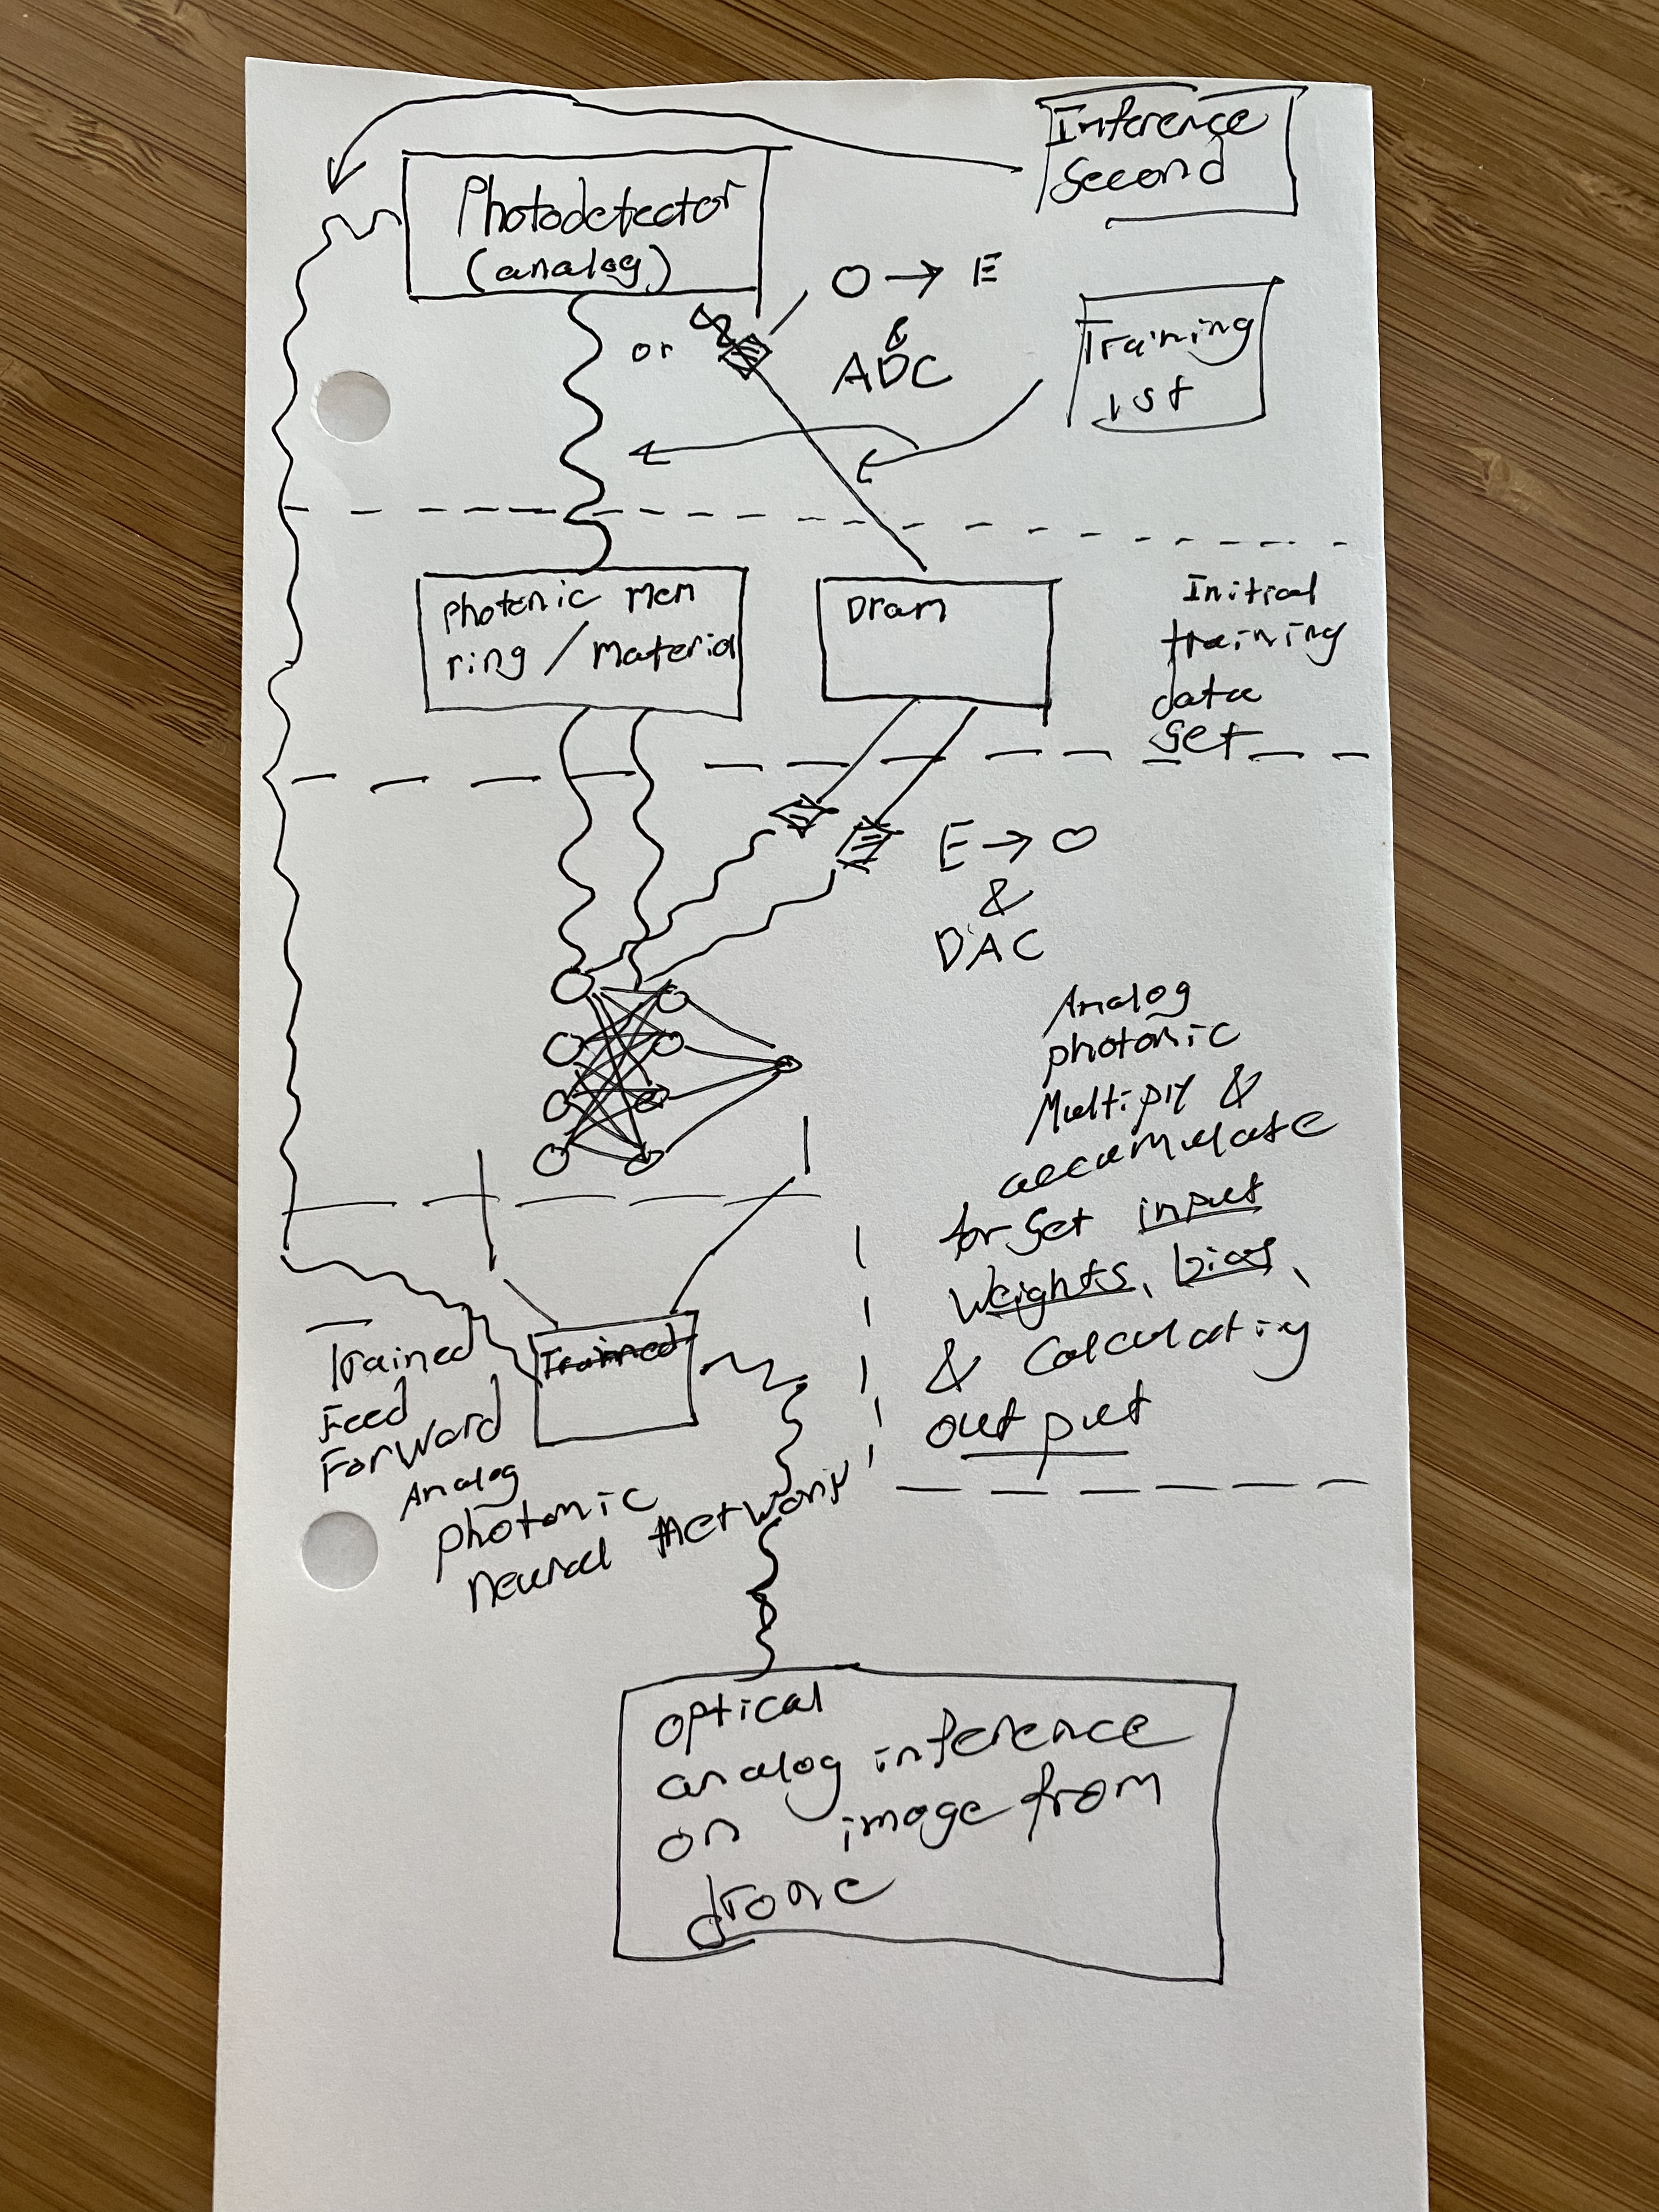
\includegraphics[height=6.0in]{figures/final/drone_arch.png}}
    \caption{Feed forward fully connected 4 input input one hidden layer one output neural network. Calculation of the forward phase for each input-output pair $\left(\vec{x}_{d}, y_{d}\right)$ and the results $\hat{y}_d$, $a_k^k$, and $o_{j}^{k}$ for each node $j$ in layer $k$ by proceeding from layer 0, the input layer, to layer $m$, the output layer.}
    \label{fig:nn architecture}
    \end{figure}


\subsection{Machine Learning}
    \begin{enumerate}
        \item Association occurs when you pick up an apple at the supermarket and squeeze it for a feeling of firmness. Previous experience tells you that firmness and freshness are correlated. The apple is firm, therefore it is fresh. \textbf{Supervised} learning occurs when you look at the apple, see that it is green, recall that green apples are most often granny smith apples, and then decide that you are looking at a granny smith apple. \textbf{Unsupervised} learning occurs when you pick up the apple, are unaware if you will like it or not, take a bite out of it, and place it in your bag if you like it, or back on the shelf if you do not. \textbf{Reinforcement} learning occurs when the store owner confronts you for all the single bite apples you have been placing on the shelf. Your knowledge of your level of physical fitness relative to store owner prompts you to make a run for it. However, your lack of knowledge of the taser equipped security guard at the store exit, resulting in a 50,000 volt signal and an alteration of state into incarceration, bestow you with new knowledge in the form of decision making weights, as your enter the showers of your new home with all of your new friends. 
        \item Input and Output
            
            \begin{itemize}[label={}]
                \item $[100,50] \rightarrow 4.55$
                \item $[105,45] \rightarrow 4.68$
                \item $[95,40] \rightarrow 4.05$
                \item $[90,50] \rightarrow 4.06$
            \end{itemize}
        
        The model is $w_1 \times \text{weight} + w_2 \times\text{diameter} + b = \text{price}$. The error function in classic backpropagation is the mean squared error shown in equation \ref{meanSquaredError}. 
        
        \begin{equation} \label{meanSquaredError}
        E(X, \theta)=\frac{1}{2 N} \sum_{i=1}^{N}\left(\hat{y}_{i}-y_{i}\right)^{2}
        \end{equation}
        
        For the first parameter set $w_1=0.05$, $w_2=0.01$, $b=-1.0$
        
        \begin{itemize}[label={}]
            \item $\hat{y}_1 = \left(0.05*100+0.01*50)+(-1) = 4.5$
            \item ${y}_1 = 4.55$
            \item $\hat{y}_2 = \left(0.05*105+0.01*45\right)+(-1) = 4.7$
            \item ${y}_2 = 4.68$
            \item $\hat{y}_3 = \left(0.05*95+0.01*40\right)+(-1) = 4.15$
            \item ${y}_3 = 4.05$
            \item $\hat{y}_4 = \left(0.05*90+0.01*50\right)+(-1) = 4$
            \item ${y}_4 = 4.05$
            \item $\text{MSE} = E(X,\theta) = \frac{1}{2N}\sum_{i=1}^{N}\left(y_i-\hat{y_i}\right)^2$
            \item $E(X,\theta) = \frac{1}{8}\left(\left (4.55-4.5\right)^2+\left(4.68-4.7\right)^2+\left(4.05-4.15\right)^2+\left(4.05-4\right)^2\right)$
            \item $E(X,\theta) = 0.001925$
        \end{itemize}
        
        For the second parameter set $w_1=0.03$, $w_2=0.03$, $b=+0.5$
        
        \begin{itemize}[label={}]
            \item $\hat{y}_1 = \left(0.03*100+0.02*50)+0.5 = 4.5$
            \item ${y}_1 = 4.55$
            \item $\hat{y}_2 = \left(0.03*105+0.02*45\right)+0.5 = 4.55$
            \item ${y}_2 = 4.68$
            \item $\hat{y}_3 = \left(0.03*95+0.02*40\right)+0.5 = 4.15$
            \item ${y}_3 = 4.05$
            \item $\hat{y}_4 = \left(0.03*90+0.02*50\right)+0.5 = 4.2$
            \item ${y}_4 = 4.05$
            \item $\text{MSE} = E(X,\theta) = \frac{1}{2N}\sum_{i=1}^{N}\left(y_i-\hat{y_i}\right)^2$
            \item $E(X,\theta) = \frac{1}{8}\left(\left (4.55-4.5\right)^2+\left(4.68-4.55\right)^2+\left(4.05-4.15\right)^2+\left(4.05-4.2\right)^2\right)$
            \item $E(X,\theta) = 0.006488$
        \end{itemize}
        
        The first set of parameters is prefered because it has a lower MSE. Back propagation can be accomplished by first calculating the forward phase for each input-output pair $\left(\vec{x}_{d}, y_{d}\right)$ and the results $\hat{y}_d$, $a_k^k$, and $o_{j}^{k}$ for each node $j$ in layer $k$ by proceeding from layer 0, the input layer, to layer $m$, the output layer. Then calculate the backward phase for each  input-output pair $\left(\vec{x}_{d}, y_{d}\right)$ and store the results $\frac{\partial E_{d}}{\partial w_{i j}^{k}}$ for each weight $w_{ij}^{k}$ connecting node $i$ in layer $k-1$ to node $j$ in layer $k$ by proceeding from layer $m$, the output layer, to layer 1, the input layer.
        
        \item Since we are using the same function between the first and second layer and the second and third layer if we had a training output value at each layer we could calculate the mean square error at each layer to see if it is decreasing or increasing. If it continues to decrease as we add more layers this is a good approach, if not, then we need to change the function to make it less continuous potentially allowing improvements in prediction without an increase in layers.
    \end{enumerate}

\subsection{Machine Intelligence in the Context of Society and your Career}
    \begin{enumerate}
        \item a) I am interested in AI's ability to make betters prediction on the behaviors of graphs. Data that is sparse and most effectively modeling in a graph based data structure teds to have a more rich representation of interactions that are driven by independent actors with a high degree of agency. Being able to make predictions off of graph traversals as opposed to immediately going to tensor based representations of data will open of this part of the AI research community. b) I think the key to avoiding redundancy as an engineering is to always have multiple skill sets your are developing and multiple classes of problems that you are working on, you sacrifice you ability to focus but you gain knowledge at the types of technologies that are developing independent of one another and it gives you an edge on how they are likely to converge to fully solve a problem and make it so there is less need (or less value add) for people to continue solving it. c) Most jobs in some ways will be impacted by AI, trying to find a niche that is not is a kin to trying to find the tallest mountain as the sea rises. You may find a dry spot but it will be crowded and you may still be submerged in the future. Better to get in the water, learn how to swim, and maybe even grow gills. 
        \item You need to know which types of decision are worth making slowly with a human in the loop because the consequences will have a large effect on peoples lives. The development of legal frame works around which decision fall into that category and how they are enforced is a good role for government to play. The market will most likely optimize for efficiency and increased productivity at the potential expense of a growing percentage of peoples well being.
    \end{enumerate}
    
\subsection{Bonus 1: Network Analysis}
    \begin{enumerate}
        \item Long Short Term Memory (LSTM) recurrent neural network
        \item Time series based predictions is one of the most common because you do not want the first events to overly influence the weights, forgetting allows for events further in time to still play an important role in altering the weights.
    \end{enumerate}

\subsection{Bonus 2: Deep Neural Networks}
    \begin{enumerate}
        \item Deep Neural Networks have multiple sets of hidden layers and depending on how connected each layer is and the changes in activation functions throughout the hidden layers play a large role in the the output layer. The hidden layers can also be feed forward or recurrent depending on the architecture. The more layers the more weights, and potentially bias you have to modify in each iteration. However deeper networks can encounter diminishing returns with each additional layer. Deep convolutional neural networks are used heavily in computer vision because of there improving performance in visual object recognition, detection, and segmentation.
    \end{enumerate}

\end{document}
